\documentclass[]{article}

\usepackage{listings}
\usepackage{color} %red, green, blue, yellow, cyan, magenta, black, white
\definecolor{mygreen}{RGB}{28,172,0} % color values Red, Green, Blue
\definecolor{mylilas}{RGB}{170,55,241}
\definecolor{cBackground}{RGB}{30,30,30}
\definecolor{cComments}{RGB}{96,139,79}
\definecolor{cStrings}{RGB}{206,145,120}
\definecolor{cKeywords}{RGB}{86,156,214}
\definecolor{cMoreKeywords}{RGB}{197,134,192}
\definecolor{cNumbers}{RGB}{181,206,168}
\definecolor{cUint}{RGB}{75,195,171}
\definecolor{cIdentifiers}{RGB}{220,220,170}
\definecolor{terminalBackground}{RGB}{62,62,62}
\definecolor{terminalDollar}{RGB}{67,103,181}
\definecolor{pythonBackground}{RGB}{39,40,34}
\definecolor{pythonComments}{RGB}{117,113,94}
\definecolor{pythonStrings}{RGB}{230,219,113}
\definecolor{pythonKeywords}{RGB}{249,38,114}
\definecolor{pythonMoreKeywords}{RGB}{155,129,223}
\definecolor{pythonFunctions}{RGB}{99,217,239}
\usepackage{graphicx}
\usepackage{etoolbox}
\usepackage{hyperref}
\usepackage{multicol}
\usepackage{fancybox}

\def\changemargin#1#2{\list{}{\rightmargin#2\leftmargin#1}\item[]}
\let\endchangemargin=\endlist

\newcommand{\docname}{Crazyflie Guide}
\newcommand{\informalname}{Drones for Dummies}
\newcommand{\typesetter}{Brian Raymond}
\newcommand{\contributors}{Tameez Latib, Joey Miller}
\newcommand{\labnames}{Prof. Tabuada's Cyber-Physical Systems Laboratory and \\Prof. Fragouli's Algorithmic Research in Network Information Flow Laboratory}

\makeatletter
\newenvironment{CenteredBox}{% 
	\begin{Sbox}}{% Save the content in a box
	\end{Sbox}\centerline{\parbox{\wd\@Sbox}{\TheSbox}}}% And output it centered
\makeatother

\lstnewenvironment{terminal}
{
	\lstset{language=bash,
		basicstyle=\color{white}\ttfamily,
		backgroundcolor=\color{terminalBackground},
		emph=[1]{\$},emphstyle=[1]{\color{terminalDollar}\ttfamily},
		breaklines=true
}}
{}

\lstnewenvironment{C}
{
	\lstset{language=C,
		basicstyle=\color{white}\ttfamily,
		backgroundcolor=\color{cBackground},
		keywordstyle=\color{cKeywords}\ttfamily,
		stringstyle=\color{cStrings}\ttfamily,
		commentstyle=\color{cComments}\ttfamily,
		emph=[1]{uint8_t, uint16_t, uint32_t},emphstyle=[1]\color{cUint}\ttfamily,
		emph=[2]{if, else, return, break, case, switch},emphstyle=[2]\color{cMoreKeywords}\ttfamily,
		breaklines=true,%
		%			identifierstyle=\color{vsIdentifiers},%
		showstringspaces=false,%without this there will be a symbol in the places where there is a space
		numbers=left,%
		numberstyle={\color{cNumbers}}\ttfamily,% size of the numbers
		numbersep=9pt, % this defines how far the numbers are from the text
}}
{}

\lstnewenvironment{Python}
{
%	\changemargin{-0.86in}{-0.86in}
	\lstset{language=Python,
		basicstyle=\small\color{white}\ttfamily,
		backgroundcolor=\color{pythonBackground},
		otherkeywords={!,!=,=,~,*,\&,+,-,^,\%,\%/\%,\%*\%,\%\%,<-,<<-,/},
		keywordstyle=\color{pythonKeywords}\ttfamily,
		emph=[1]{None,True,False},emphstyle=[1]\color{pythonMoreKeywords}\ttfamily,
		stringstyle=\color{pythonStrings}\ttfamily,
		commentstyle=\color{pythonComments}\ttfamily,
		emph=[2]{append, pop, min, max, add_variable, def, print, exit, len, add_config, format, add_callback, exists, open, makedirs, writer, writerow, set_value, set_setpoint, int, range, cos, sin, range, send_setpoint, sleep, send_hover_setpoint, send_position_setpoint, init_drivers, scan_interfaces, reset_estimater, begin_logging, loco_follow_paths, pos_follow_paths, vel_follow_paths, format},emphstyle=[2]\color{pythonFunctions}\ttfamily,
		breaklines=true,%
		%			identifierstyle=\color{vsIdentifiers},%
		showstringspaces=false,%without this there will be a symbol in the places where there is a space
		numbers=left,%
		numbersep=9pt, % this defines how far the numbers are from the text
		}}
{}

\begin{document}
	
\begin{titlepage}
	\begin{center}
		{\LARGE \textsc{\docname \\ (AKA \informalname)} \\ \vspace{4pt}}
		\rule[13pt]{\textwidth}{1pt} \\
		\includegraphics[width=1\linewidth]{DronesforDummies.jpg} \\
		{\vspace{1em} \large Typeset by \typesetter,\\ Contributed to by \contributors \\ \vspace{10pt}
			Under the guidance of:\\ \labnames \\ \vspace{10pt}
			\today \\ \vspace{10pt}
		}
	\end{center}
\end{titlepage}


% END TITLE PAGE %%%%%%%%%%%%%%%%%%%%%%%%%%%%%%%%%%

\cleardoublepage
\setcounter{page}{1}

\tableofcontents
\newpage

\changemargin{-1in}{-1in}

\section{Native Installation}
\subsection{Crazyflie Python Library}
\noindent In terminal, type the following to install cflib:
	
\begin{terminal}
$ git clone https://github.com/bitcraze/crazyflie-lib-python.git
$ pip install -e path/to/cflib
\end{terminal}

\noindent To use USB radio without being root:
	
\begin{terminal}
$ sudo groupadd plugdev
$ sudo usermod -a -G plugdev <username>
\end{terminal}

\noindent You will also either need to create or edit the following file:
	
\begin{terminal}
# /etc/udev/rules.d/99-crazyradio.rules
SUBSYSTEM=="usb", ATTRS{idVendor}=="1915", ATTRS{idProduct}=="7777", MODE="0664", GROUP="plugdev"
# to connect Crazyflie 2.0 via usb
SUBSYSTEM=="usb", ATTRS{idVendor}=="0483", ATTRS{idProduct}=="5740", MODE="0664", GROUP="plugdev"
\end{terminal}

\subsection{Crazyflie Python Client}
\noindent To install the client, clone the following repo and install:

\begin{terminal}
$ git clone https://github.com/bitcraze/crazyflie-clients-python.git
$ sudo apt-get install python3 python3-pip python3-pyqt5 python3-pyqt5.qtsvg
$ pip3 install -e .
\end{terminal}

\subsection{Crazyflie Firmware}
\noindent To install the Crazyflie 2.0 firmware and be able to edit it:

\begin{terminal}
$ git clone https://github.com/bitcraze/crazyflie-firmware.git
$ sudo add-apt-repository ppa:terry.guo/gcc-arm-embedded # For ubuntu 14.04 64b
$ sudo add-apt-repository ppa:team-gcc-arm-embedded/ppa # For ubuntu 16.04 64b
$ sudo apt-get update
$ sudo apt-get install libnewlib-arm-none-eabi
\end{terminal}

\noindent Compiling is done with `make'

\subsection{Crazyflie LPS Node Firmware}
\noindent To install the location positioning system (LPS) firmware and be able to edit it:

\begin{terminal}
$ git clone https://github.com/bitcraze/lps-node-firmware.git
$ sudo apt-get install libncurses5:i386
$ sudo apt-get install gcc-arm-none-eabi
\end{terminal}

\noindent Compiling is done with `make'

\section{VM Installation and Software}
\subsection{Installation}
\noindent In order to get the Crazyflie in the air quickly, Bitcraze has set up its own Virtual Machine that is preloaded with all the essential software and code necessary to begin flying the Crazyflie. The virtual machine is intended to be run in \href{https://www.virtualbox.org/}{Oracle VirtualBox}. If you wish to run the VM in \href{https://www.vmware.com/products/workstation-player.html}{WMPlayer} you will need to install some \href{https://www.vmware.com/support/ws5/doc/ws_newguest_tools_linux.html#wp1118025}{additional tools} yourself. The Virtual Machine itself has an \href{https://wiki.bitcraze.io/projects:virtualmachine:index}{online index}. If you wish to get the latest version of the VM, it can be found on their \href{https://github.com/bitcraze/bitcraze-vm/releases/}{VM release page} on Github. \\

\noindent One error that may come up iswhen running the VM will say something to the effect that there is an issue with the USB controller. To fix this, be sure to select the USB 1.1 OHCI configuration. Once this is done, the virtual machine should hopefully install and boot smoothly. Once it finishes installing, boot up the VM and click on the desktop configuration file named Update all Projects to automatically update all Crazyflie Github Repos. The Following is all the information necessary about the VM. It can also be found in the README on the Desktop of the VM. \\
\begin{terminal}
* The username is: bitcraze
* The password is: crazyflie
* The virtual machine has 30GB drive and 1 GB of RAM
* The virtual machine is using Xubuntu 14.04.4 LTS
\end{terminal}

\subsection{Installed Software}
\noindent The following software has been pre-installed (besides basic setup)
\begin{multicols}{2}
\begin{itemize}
\item Virtualbox guest additions
\item gnu-arm-none-eabi + build tools
\item Git
\item gitg
\item PyCharm
\item Oracle Java JRE (for PyCharm)
\item pyusb, pygame and pyqt
\item PyQtGraph
\item Qt4 and Qt Designer
\item KDE Marble with Python-bindings
\item KiCad
\item Eclipse with compiling/debugging/flashing
\item Leafpad
\item EmbSys RegView for Eclipse
\item dfu-util
\end{itemize}
\end{multicols}

\subsection{System tweaks}
\noindent The udev rules to access the Crazyradio and the NRF bootloader have been added to the udev configuration. They have also been added to the Virtual Box pre-set filters.

\subsection{Projects}
\noindent The following projects have been pre-cloned into the /home/bitcraze/projects directory:

\begin{multicols}{2}
\begin{itemize}
\item crazyflie-pc-client
\item crazyflie-firmware
\item crazyflie-bootloader
\item crazyradio-firmware
\item crazyradio-electronics
\item crazyflie2-nrf-firmware
\item crazyflie2-stm-firmware
\item crazyflie2-stm-bootloader
\end{itemize}
\end{multicols}

\section{Running Crazyflie}

\subsection{PC Client}
\noindent The Crazyflie PC client can be run by using the following command:


\begin{terminal}
# On virtual machine:
$ python3 /home/bitcraze/projects/crazyflie-pc-client/bin/cfclient
# On native install:
$ cfclient
\end{terminal}

\noindent Or by using the shortcut on the desktop.

\noindent {\bfseries Please note:} If no other input device is passed to the VM the ``VirtualBox USB Tablet" device will be used. Do not connect to the Crazyflie using this device, since the thrust will then be controlled by the mouse movements on the screen.


\subsection{Updating Repos}
\noindent Updating to the latest versions of all the repositories can be done by using the following:

\begin{terminal}
# On virtual machine:
$ /home/bitcraze/bin/update_all_projects.sh
# On native install:
$ /home/desiredRepoToUpdate git pull
\end{terminal}

On the virtual machine, the shortcut on the desktop may also be used.

\subsection{Updating Crazyradio Firmware}
\noindent Download the latest firmware and run the following commands:
% Add link?

\begin{terminal}
$ cd /home/bitcraze/projects/crazyradio-firmware
$ python usbtools/launchBootloader.py
\end{terminal}

\noindent If you have not activated the USB filter for the NRF bootloader, pass the newly
found "NRF BOOT" USB device to the virtual machine and then run the following
command:

\begin{terminal}
$ python usbtools/nrfbootload.py flash new_firmware_file.bin
\end{terminal}

\subsection{Compiling Crazyflie Firmware} \label{ss: crazyflie-firmware-flash}
\noindent A version of the Crazyflie firmware that is upgradable using the Crazyradio bootloader can be built using the following commands:

\begin{terminal}
$ cd /InstallLocation/crazyflie-firmware
$ make CLOAD=1 DEBUG=0
\end{terminal}

\noindent This firmware can then be downloaded to the Crazyflie using the cfclient or the ``Flash using radio" make target in Eclipse.

\subsection{Adding USB Drivers}

\noindent Finally, be sure to right-click on the USB at the bottom of the Virtual Machine and select USB Settings. This will allow you to add USB drivers to the VM and is necessary to run a controller for flying the drone or allow it to recognize the CrazyRadio Dongle.

\subsection{Bootloading the Crazyflie}

\noindent Once the Drone has been assembled, it is necessary to flash the \href{https://github.com/bitcraze/crazyflie-release/releases}{latest
firmware} onto the drone itself. Select the latest release zip file and use it for bootloading. To bootload the Crazyflie, hold the power button for 3 seconds and it should begin to flash blue LED's. If it makes the ordinary startup jingle and rotates its motors, turn it off and try again. Open up the CFClient and click on the connect tab on the top to open a drop down menu. Select Bootloader and then click on Initiate bootloader cold boot in the new window. It should connect to the Crazyflie. Once it is connected, click on browse and select the zip file you previously downloaded. Now click program and wait for it to finish flashing the firmware. once it has completed, be sure to click restart in firmware mode. Failure to do so will result in the Crazyflie not being updated to the new firmware.

\section{Custom Firmware}

\subsection{Crazyflie}

\noindent If the project you are currently working on requires you to modify the firmware, there are two repositories you will need to focus on. The first is the
\href{https://github.com/bitcraze/crazyflie-firmware}{Crazyflie 2.0 Firmware} and the second is the \href{https://github.com/bitcraze/crazyflie2-nrf-firmware}{Crazyflie 2.0 NRF Firmware}. Clone these repositories and make your modifications as necessary. Once you are finished, run the make file and copy the binary created. The zip file downloaded in the last section contains 2 binaries and a json file. The json file specifies the names of the binaries so it is easiest to rename the binaries you generate from the make to the names of the binaries in the zip, extract the json file and then zip them up to create your new firmware package. The binaries are thankfully named appropriately such that it is easy to tell which one corresponds to NRF and the one for the ordinary firmware. Once you have your new zip file, follow the same steps in the section on Bootloading the drone to flash your modified firmware to the drone itself.

\subsection{Loco-Positioning System}

\noindent To modify the firmware for the LPS system, you will need to modify the \href{https://github.com/bitcraze/lps-node-firmware}{lps node firmware} repository and upload it the node using \href{https://github.com/bitcraze/lps-tools}{lps tools}. \\

\noindent To install and run lps tools:

\begin{terminal}
# To install, navigate to cloned folder and type:
$ pip3 install -e .[pyqt5]
# To run:
$ python3 -m lpstools
\end{terminal}

\noindent If trying to modify the firmware on 64bit Linux, make sure you have the following 32bit libraries:

\begin{terminal}
$ sudo apt-get install libncurses5:i386	
\end{terminal}

Then once files are modified, run the following in the root directory and upload the `.dfu' in `lps-node-firmware/bin' with lpstools:

\begin{terminal}
$ make clean; make
\end{terminal}

\section{Debugging}

\subsection{Crazyflie Firmware Debugging}

\noindent For debugging the Crazyflie, the \href{https://www.bitcraze.io/debug-adapter-kit/}{debug adapter} sold through bitcraze and a \href{https://www.mouser.com/ProductDetail/STMicroelectronics/ST-LINK-V2?qs=H4BOwPtf9MC1sDQ8j3cy4w\%3D\%3D\&gclid=Cj0KCQjw77TbBRDtARIsAC4l83n7YmsHaUOhIKdwmhN99Ryz07R8_PLHcgRH1x0KDGkoEPuFHsZZVjsaAgH9EALw_wcB}{ST-Link/v2} will be needed. To install the proper ST-Link v2 drivers, do the following:

\begin{terminal}
$ git clone https://github.com/texane/stlink stlink.git
$ cd stlink
$ make
# install binaries
$ sudo cp build/Debug/st-* /usr/local/bin
# install udev rules
$ sudo cp etc/udev/rules.d/49-stlinkv* /etc/udev/rules.d/
# restart udev rules
$ sudo restart udev
\end{terminal}

\noindent Also be sure to install \href{https://www.eclipse.org/downloads/download.php?file=/oomph/epp/photon/R/eclipse-inst-linux64.tar.gz}{Eclipse Photon} and \href{https://gnu-mcu-eclipse.github.io/openocd/install/#gnulinux}{openOCD} both on-system and within Eclipse as a debugging plugin (reference link for both).

\subsubsection{STM32}

Within Eclipse: \\
Go to `Run' $\rightarrow$ `Debug Configuration'. Create a new `GDB OpenOCD Debugging' configuration and call it `Crazyflie 2.0 STM32.' \\

Under Main: \\
Make `Project' your firmware folder and `C/C++ Application' your cf2.elf file. Within `Build (if required) before launching' section set `Build Configuration' to `Select Automatically' and click on `Use workspace settings'.

\includegraphics[width=0.55\linewidth]{DebugConfig1.png}

Under Debugger: \\
Within `OpenOCD Client Setup' section ensure that executable is `\$\{openocd\_path\}/\$\{openocd\_executable\}', `GDB port' is 3333, `Telnet port' is 4444, and `Config options' are ` -f ``board/stm32discovery.cfg" '. \\
Within `GDB Client Setup' ensure that `Executable' is `/usr/bin/arm-none-eabi-gdb' and the `Commands' are `set mem inaccesible-by-default off'.

\includegraphics[width=0.55\linewidth]{DebugConfig2.png}

Under Startup: \\
Ensure it is the same as the following.

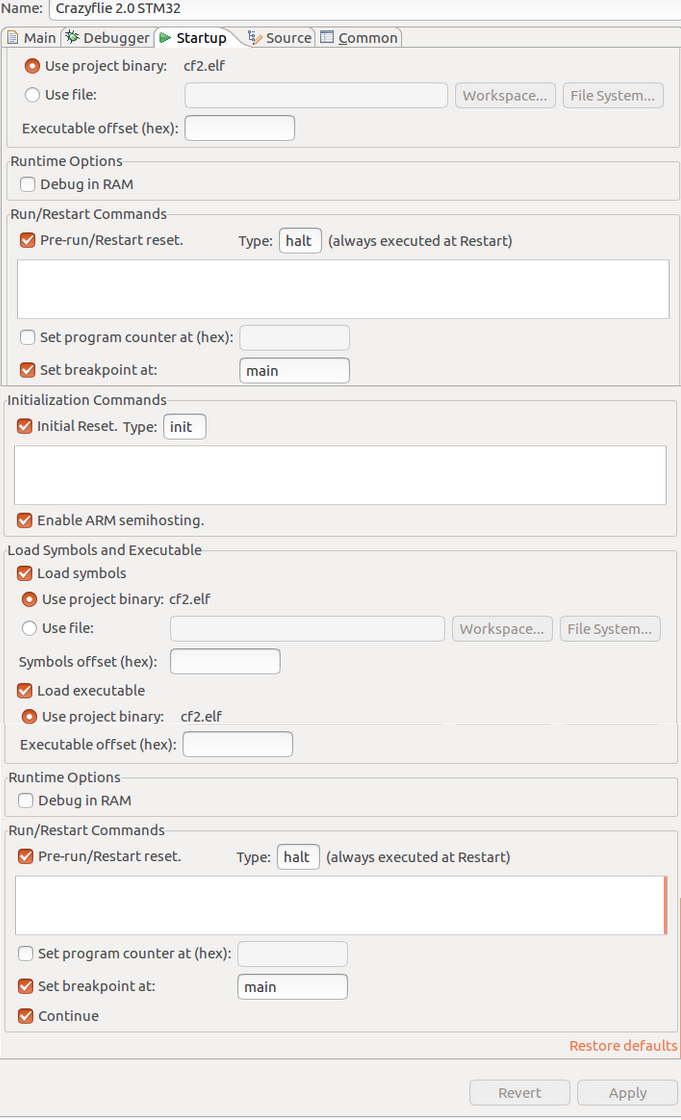
\includegraphics[width=0.55\linewidth]{DebugConfig3.png}

\newpage

Under Common: \\
Within `Save as' section check `Shared file' and set the location to the folder of the crazyflie firmware.

\includegraphics[width=0.55\linewidth]{DebugConfig4.png}

Under the Build Targets view add the following targets by clicking `New Build Target':
``Make CLOAD DEBUG" with the parameters ``all CLOAD=1 DEBUG=1"
``Make CLOAD" with the parameters ``all CLOAD=1 DEBUG=0"
``Make DEBUG" with the parameters ``all CLOAD=0 DEBUG=1"
``Flash using debugger" with parameters ``flash"
``Flash using radio" with parameters ``cload"


To run the debugger within Eclipse:\\
$>$ Make DEBUG \\
$>$ Flash using debugger \\
$>$ Run $\rightarrow$ Debug Configurations $\rightarrow$ Crazyflie 2.0 STM32 $\rightarrow$ Debug

\subsubsection{nRF51}

\noindent Currently unsure how to debug.

\subsection{Crazyflie Python Lib}

The debugging of the python code is a lot simpler as you can just use the python debugger (pdb) library.

This can be done by either running the following terminal command:

\begin{terminal}
$ python -m pdb myscript.py
\end{terminal}

Or adding `import pdb; pdb.set\_trace()' where you want to break the file you wish to debug and then running the file via terminal.

Within terminal, these are key commands:
\begin{terminal}
$ h # help
$ l # list code around current break
$ s # step to next executed line
$ n # step to next line in current file
$ c # continue to next breakpoint
\end{terminal}

\subsection{ROS}

\section{Loco-Positioning System}

\subsection{Configuring Drones}

\noindent To install the Loco-Positioning deck onto the Crazyflie, be sure to place the flat end of the deck that has the `0xBC' logo face down over the battery. The drone must be powered off while installing and removing the deck. Push all the pins through the inserts on the deck and it should now be ready to use with the Loco-Positioning System (LPS). \\

{\bfseries Note:} We found that for the Crazyflie to work, we needed to re-flash (see Section \ref{ss: crazyflie-firmware-flash}) the firmware as the drone is only configured for currently connected decks (e.g. flow deck and LPS deck). \\

\subsection{Configuring Nodes}

\noindent To flash node firmware to the Loco-Positioning Nodes, you will need to install the LPS configuration tool. Clone the following \href{https://github.com/bitcraze/lps-tools}{Git Repository} and follow the instructions in the README. If you are running Windows on your device, you can alternatively install it by downloading the \href{https://github.com/bitcraze/lps-tools/releases}{lps-tools-win32-install file}. Once you have installed the configuration tool, you must download the \href{https://github.com/bitcraze/lps-node-firmware/releases}{firmware for the nodes}. Select the .dfu file. To update the node, open up the LPS configuration tool and plug in the node via USB while holding down the button labeled DFU. If on Windows, you will need to \href{https://wiki.bitcraze.io/misc:usbwindows}{follow instructions} on installing the nodes USB driver with Zadig. In the client, click on the browse button and select the firmware file you recently downloaded. Now click update and finally press the reset button on the node once it completes the update. Once all the nodes are updated, connect them to the computer normally and configure the ID. If you wish to operate in TWR mode, make sure the Mode is set to Anchor (TWR). Click apply and assign every node a different ID. Mark them with electrical tape or some other method to easily keep track of the IDs of the nodes.

\subsection{Node Placement}

\noindent Place the anchors in the room at least 2 meters apart with a line of site to the flying volume. For TWR Mode, 4 anchors is the minimum with 6 being ideal and 8 if redundancy is needed.

\section{Setpoint Following}

\subsection{Setup}

\noindent To accomplish this, we used the Crazyflie2.0 with the `Flow deck' %add link
 and the `Loco-Postioning deck' %add link
 as the flow sensor aides in velocity/ height calculations while the loco-positoning deck aides in absolute position calculations. This is all done with Bitcraze's internal kalman filter and pid functions which are a part of the crazyflie firmware code.
 
\subsection{Code}

\noindent For setpoint following we heavily modified Luigi Pannochhi's code which utilizes the built-in commander python library provided by bitcraze. The python script takes in an input to specify which type of path following it should use: `l' for loco-positioning based, `p' for positioning based, and `v' for velocity based. The names are a little deceiving, however, as both `l' and `p' use the beacons. The difference between the two is that `l' creates setpoints internally using thrust, roll, pitch, and yaw while `p' creates setpoints using x, y, z, and yaw.\\

\noindent The following is a look at each of these setpoint following functions. Note that there are globals DT, T, VMAX, and START\_HEIGHT. DT is the default dT for go\_straight\_d, T is the default time of flight, VMAX is the maximum velocity limit, and START\_HEIGHT is the initial hover height.

\newpage
\begin{Python}
def go_straight_d(cf, d_x, d_y, z, t, dt=DT):
	if (t == 0):
		return
	steps = int(t/dt)
	v = [d_x/t, d_y/t]
	for r in range(steps):
		cf.commander.send_hover_setpoint(v[0], v[1], 0, z)
		time.sleep(dt)

def loco_follow_paths(scf):
	cf = scf.cf
	cf.param.set_value('flightmode.posSet', '1')
	for position in sequence:
		for i in range(200):
			cf.commander.send_setpoint(position[1], position[0],
					position[3], int(position[2] * 1000))							
		time.sleep(0.01)
	time.sleep(0.1)

def pos_follow_paths(scf):
	cf = scf.cf
	cf.param.set_value('flightmode.posSet', '1')
	cf.commander.send_hover_setpoint(0,0,0,START_HEIGHT)
	time.sleep(1)
	cf.commander.send_position_setpoint(0,0,START_HEIGHT,0)
	time.sleep(1)
	for position in sequence:
		cf.commander.send_position_setpoint(position[0], position[1],
		position[2], 0)
		time.sleep(1)

def vel_follow_paths(scf):
	cf = scf.cf
	cf.param.set_value('flightmode.posSet', '1')
	cf.commander.send_hover_setpoint(0,0,0,START_HEIGHT)
	time.sleep(1)
	movement = sequence[0]
	for position in sequence:
		movement = (position[0]-position_internal[0], 
					position[1]-position_internal[1], 
					position[2], position[3])
		t = T
		if (abs(movement[0]/T) > VMAX or abs(movement[1]/T) > VMAX):
			t = abs(movement[0]/VMAX) if abs(movement[0]/VMAX) > 
				abs(movement[1]/VMAX) else abs(movement[1]/VMAX) 
		go_straight_d(cf, movement[0], movement[1], movement[2], t)
		time.sleep(1)
		for i in range(4):
			position_internal[i] = position[i]
		time.sleep(0.1)
\end{Python}

\section{Logging}

\subsection{Loggable Variables}

% TODO: Add a reference to opening the cfclient
\noindent To see all the variables which can be logged, open the cfclient, connect to the crazyflie, and enable the Log TOC by selecting `View $\rightarrow$ Tabs' in the top menu bar and checking the box next to `Log TOC.' This should then enable the following tab, which may be perused to see all variables logged by each of the key words.

\includegraphics[width=1\linewidth]{TOCList.png}

Logging is done by creating a LogConfig with the name of the measurement to be recorded, and then adding variables with the names formatted according to the Log TOC.

\subsection{Skeleton Code}

\begin{Python}
import cflib
import logging
from cflib.crazyflie.log import LogConfig

dataLog = errorLog = pos_writer = log_timestamp = log_conf = Logger = None

def begin_logging(cf):
	global Logger	
	Logger = SkeletonLogger(cf)
	Logger.start_logging()

class SkeletonLogger:
	def __init__(self, cf):	
		self.cf = cf
		logging.basicConfig(level=logging.ERROR)

	def start_logging(self):
		global pos_writer
		pos_log_file = open(self.directory + self.log_timestamp 
			+ '_pos.csv', 'wb')
		pos_writer = csv.writer(pos_log_file)
		pos_writer.writerow(['time', 'x_pos', 'y_pos', 'z_pos'])
		log_pos = LogConfig(name='Position', period_in_ms=10)
		
		try:
			log_pos.add_variable('kalman.stateX', 'float')
			log_pos.add_variable('kalman.stateY', 'float')
			log_pos.add_variable('kalman.stateZ', 'float')
			self.cf.log.add_config(log_pos)
			# This callback will receive the data
			log_pos.data_received_cb.add_callback(print_pos)
			# This callback will be called on errors
			log_pos.error_cb.add_callback(log_error)
			# Start the logging
			log_pos.start()
		except KeyError as e:
			print('Could not start log configuration,'
				'{} not found in TOC'.format(str(e)))
		except AttributeError:
			print('Could not add Position log config, bad configuration.')
		
	def print_pos(timestamp, data, self):
		print([timestamp, data['kalman.stateX'], data['kalman.stateY'],
			data['kalman.stateZ']])
	
	def log_error(self, logconf, msg):
		"""Callback from the log API when an error occurs"""
		print('Error when logging %s: %s' % (logconf.name, msg))
		if self.errorLog == None:
			if not os.path.exists(DIRECTORY):
				os.makedirs(DIRECTORY)
			self.errorLog = open(DIRECTORY + datetime.datetime.now().strftime("Error Log %Y-%m-%d_%H:%M:%S"), 'a')
		else:
			self.errorLog.write('Error when logging %s: %s\n'
				% (logconf.name, msg))
\end{Python}

\noindent This code may be copy/pasted into a python script, and the begin\_logging function be called by passing a Crazyflie handle. Note that if using a SyncCrazyflie handle called `scf,' one should instead pass `scf.cf' to begin\_logging. \\

\subsection{AltLogger}

\noindent AltLogger.py is the robust, custom logger class that we created. To use, simply put `include AltLogger as AltLogger' in your python script header, and then once having created the Crazyflie handle, call AltLogger.begin\_logging(). Called with just the Crazyflie handle, this function saves data about stability, position, acceleration, and gyroscope to .csv files in a folder called `/LoggedData/' in the same directory as file being ran. The following is the header for the function:

\begin{Python}
allowedItems = ['stab', 'pos', 'acc', 'gyro']
defaultPath = './LoggedData/'
	
def begin_logging(handle, arg1=None, arg2=None)
# By default, arg1 = allowedItems and arg2 = defaultPath
# To pass something other than allowedItems, pass a list subset of allowedItems
# To pass something other than defaultPath, pass a string that is a valid file path
# Note: None, either, or both of these may be passed, order independent
\end{Python}

\section{Custom Communication}

\subsection{\texorpdfstring{Crazyflie $\rightleftharpoons$ Base Station}%
	{Between Crazyflie and Base Station}}

\subsubsection{Crazyflie Code}

\noindent When consoleCommInit is called, it creates the header for our CRTP packet and this allows us to direct it at a particular port. It also creates a new task/process. This process will block until it receives a packet with the right header. Then, we can interpret this custom data from the PC. In the sample code, we also call consoleCommPuts, which puts a string into the buffer ready to be sent and consoleCommPflush, which puts and flushes.

\begin{C}
// consoleComm.c

void consoleCommInit() {
	if (isInit) return;
	messageToPrint.size = 0;
	messageToPrint.header = CRTP_HEADER(CRTP_PORT_CONSOLE, 0);
	vSemaphoreCreateBinary(consoleLock);
	xTaskCreate(consoleCommTask, CONSOLE_COMM_TASK_NAME,
	CONSOLE_COMM_TASK_STACKSIZE, NULL, CONSOLE_COMM_TASK_PRI);
	isInit = true;
	consoleCommPflush("Console Comm init!");
}
\end{C}

\newpage
\begin{C}
// consoleComm.c

void consoleCommTask(void * prm) {
	crtpInitTaskQueue(CRTP_PORT_CONSOLE);
	
	while(1) {
		crtpReceivePacketBlock(CRTP_PORT_CONSOLE, &messageReceived);
		
		// process data in messageReceived.data
	}
}
\end{C}

\subsubsection{Base Station Code}

\noindent For the Base Station to communicate it needs to send a packet to the drone using the CRTProtocol. We included this in the commander class but it could be done anywhere with the correct includes.

\begin{Python}
def send_message(self, str):
	for i in range(len(str)/29 + 1):
		pk = CRTPPacket()
		pk.port = CRTPPort.DRONE
		pk.data = struct.pack('<30s', str[29*i:(30*(i+1))-(i+1)])
		self._cf.send_packet(pk)
\end{Python}

\subsection{\texorpdfstring{Crazyflie $\rightleftharpoons$ Beacon}%
	{Between Crazyflie and Beacon}}

\subsubsection{Crazyflie Code}

When the drone receives a packet from the beacon we check the type of packet it is. If it is of type LPS\_TWR\_RELAY\_B2D (B2D = Beacon to Drone), then we can process it within beaconComm's analyzePayload() function. Currently, we have this function make a call to consoleCommPflush().

\begin{C}
// lpstwrtag.c
case LPS_TWR_RELAY_B2D:
{
	beaconAnalyzePayload((char*)rxPacket.payload);
	ranging_complete = true;
	messageToSend = 0;
	messageExpected = 0;
	return 0;
	break;
}
\end{C}

Note that in sendMessageToBeacon(), we set the  messageToSend flag which tells lpstwrtag.c to communicate our custom messages instead of its normal poll $\rightarrow$ ans $\rightarrow$ final $\rightarrow$ report routing. Within the CRTPPAcket we set the header to LPS\_TWR\_RELAY\_D2B instead of LPS\_TWR\_POLL which is just a \#define.

\begin{C}
// lpstwrtag.c
void initiateRanging(dwDevice_t *dev) {
//	...
	if (messageToSend) {
		messageExpected = 1;
		memcpy(txPacket.payload, message, LPS_MAX_DATA_SIZE);
		txPacket.payload[LPS_TWR_TYPE] = LPS_TWR_RELAY_D2B;
	}
	else {
		txPacket.payload[LPS_TWR_TYPE] = LPS_TWR_POLL;
	}
	txPacket.payload[LPS_TWR_SEQ] = ++curr_seq;
	txPacket.sourceAddress = options->tagAddress;
	txPacket.destAddress = options->anchorAddress[current_anchor];
	dwNewTransmit(dev);
	dwSetDefaults(dev);
	dwSetData(dev, (uint8_t*)&txPacket, MAC802154_HEADER_LENGTH+2+28);
//	...
}
\end{C}

The file/header pair beaconComm has functions similar to those of consoleComm, but on beaconCommFlush (and the subsequent call to  beaconCommSendMessage) it puts the data into a buffer in lpstwrtag, which will be sent on the next communication cycle between the beacon and drone.

\begin{C}
// beaconComm.c
static bool beaconCommSendMessage(void) {
	sendMessaeToBeacon(message);
	consoleCommPflush(message);
	messageLength = 2;
	// First byte is the header, and the second is the sequence number
	return true;
}
//	...
void sendMessageToBeacon(char * msg) {
	messageToSend = 1;
	consoleCommPflush(msg);
	memcpy(message, msg, LPS_MAX_DATA_SIZE);
}
\end{C}

\subsubsection{Beacon Code}

On the beacon's side of the firmware, we just modified uwb\_twr\_anchor.c to listen for the header which specifies the packet as being a part of our custom communication. Note that RELAY\_D2B is defined the same as LPS\_TWR\_RELAY\_D2B in the Crazyflie side of the firmware. RELAY\_B2D signifies the packet as being from the Beacon to the Drone (Crazyflie).

\begin{C}
// uwb_twr_anchor.c
case RELAY_D2B:
{      
	txPacket.payload[TYPE] = RELAY_B2D;
	txPacket.payload[SEQ] = rxPacket.payload[SEQ];
	memcpy(receivedMsg, rxPacket.payload + 2, PAYLOAD_LENGTH - 2);
	
	// do something to process the data
	
	dwNewTransmit(dev);
	dwSetDefaults(dev);
	dwSetData(dev, (uint8_t*)&txPacket, MAC802154_HEADER_LENGTH+2+PAYLOAD_LENGTH);
	
	dwWaitForResponse(dev, true);
	dwStartTransmit(dev);
	
	break;
}
\end{C}

\subsection{\texorpdfstring{Crazyflie $\rightleftharpoons$ Crazyflie}%
	{Between Crazyflie and Crazyflie}}

\noindent Under progress

\end{document}